\documentclass[twocolumn]{article}
\usepackage[english]{babel}
\usepackage[utf8]{inputenc}
\usepackage{amsmath,amssymb,physics,mathtools,blindtext,graphicx,float}
\usepackage[a4paper,total={7.5in,10in}]{geometry}
\usepackage[labelfont=bf]{caption}

\begin{document}
\begin{large}
\section*{Solving the radial wavefunction using B-splines}
In this report, a description will be given on how the radial function for hydrogen-like atoms,
\begin{equation}
    \label{27apr1633}
    \begin{split}
        &-\frac{\hbar^2}{2\mu}\left(\frac{1}{r^2}\left(r^2\frac{\partial R_{n\ell}}{\partial r}\right)-\frac{\ell(\ell+1)}{r^2}R_{n\ell}\right) \\ 
        &\hspace{2cm} +V(r)R_{n\ell} = ER_{n\ell},
    \end{split}
\end{equation}
is solved using B-splines. Here $R_{n\ell}(r)$ is the radial function, $\mu$ is the reduced mass, $n$ is the principal quantum number and $\ell$ is the azimuthal quantum number. This equation can be simplified by introducing the reduced radial wavefunction $P_{n\ell}(r) = rR_{n\ell}(r)$:
\begin{equation}
    \label{26apr0749}
    \begin{split}
        &-\frac{\hbar^2}{2\mu}\frac{\text{d}^2P_{n\ell}}{\text{d}r^2} + \frac{\hbar^2\ell(\ell+1)}{2\mu r^2}P_{n\ell} \\ 
        &\hspace{2.1cm} + V(r)P_{n\ell} = EP_{n\ell}.
    \end{split}
\end{equation}
The boundary conditions of $P_{n\ell}$ are $P_{n\ell}(0) = 0$ and $P_{n\ell}(r\to\infty) = 0$. The potentials which were used were the Coulomb potential:
\begin{equation}
    V_C = -\frac{Ze^2}{4\pi\epsilon_0r}
\end{equation}
and the potential from a  uniformily charged shell of radius $R_0$:
\begin{equation}
    V_S(r) = 
    \begin{cases}
        -Ze^2(3-(r/R_0)^2)/(8\pi\epsilon_0R_0), \quad r<R_0, \\ 
        -Ze^2/(4\pi\epsilon_0r), \quad r\geq R_0.
    \end{cases}
\end{equation}

\subsection*{Numerical set-up and method}
The following dimensionless variables were defined:
\begin{equation}
    \begin{split}
        &\xi = r/Da_0, \\ 
        &E' = E/\left(Z^2\mu\hbar^2/(2m_e^2a_0^2)\right).
    \end{split}
\end{equation}
In principle, $E'$ should take the values $-1,-1/4,-1/9,\dots$ for bound states. The variable $\xi$ is on the interval $[0,1]$ and $D$ is chosen so that the wavefunction is negliably small in the vicinity of $\xi=1$. Using these variables, equation \eqref{26apr0749} can be written
\begin{equation}
    \label{20apr0705}
    \hat{H}u = -\beta^2\left(\frac{\text{d}^2}{\text{d}\xi^2}-\frac{\ell(\ell+1)}{\xi^2}+\frac{2}{\beta\xi}\right)u = E'u
\end{equation}
where $\beta = m_e/(Z\mu D)$. The numerical solution to \eqref{20apr0705} is written as a linear combination of $n$ B-splines of degree $k$:
\begin{equation}
    \label{28apr1521}
    u(\xi) = \sum_{j=0}^{n-1}c_jB_{j,k}(\xi).
\end{equation}
The boundary conditions $u(0) = u(1) = 0$ are satisfied by placing $k+1$ knot points at $\xi=0$ and another $k+1$ knot points at $\xi=1$. This makes $B_{0,k}$ the only non-zero B-splines at $\xi=0$ and $B_{n-1,k}$ the only non-zero B-spline at $\xi = 1$. The boundary conditions were thus satisfied by setting $c_0 = c_{n-1} = 0$. Since the wavefunction is vanishing for $\xi$ closer to one, the inner knot points were distributed non-uniformily on the interval so that more knot points were closer to $\xi=0$ than $\xi=1$. A distribution which worked quite well was $2^{\xi^2}-1$. 

Inserting \eqref{28apr1521} into \eqref{20apr0705}, multiplying by $B_{i,k}(x)$ and integrating over $(0,1)$ yields:
\begin{equation}
    \sum_{j=1}^{n-2}c_j\int\limits_0^1B_{i,k}\hat{H}B_{j,k} = E'\sum_{j=1}^{n-2}c_j\int\limits_0^1B_{i,k}B_{j,k}
\end{equation}
which is a generalized eigenvalue problem of the form $A\mathbf{c} = E'B\mathbf{c}$. This was solved with an inverse power method, $(A-E^*B)\mathbf{c}_{j+1} = B\mathbf{c}_j$ where $E^*$ is a guess at an eigenvalue and $\mathbf{c}_j$ is normalized in each iteration. The iteration was carried out until the error $|A\mathbf{c}-E^*B\mathbf{c}|_\text{max}$ was sufficiently small ($<10^{-6}$). The elements of the matrices $A$ and $B$  were obtained by integrating with gaussian quadrature of order $d$,
\begin{equation}
    \int_{-1}^1f(x)dx \approx\sum_{j=0}^{d-1}c_jf(x_j),
\end{equation}
where $x_k$ are the Legendre roots and $c_k$ are the corresponding weights, which depend on the degree used. Since $B_{i,k}$ is non-overlapping with $B_{j,k}$ if $|j-i|>k$, it was only necessary to integrate over segments of $(0,1)$. Each such segment was divided into 20 subsegments over which the integrals were transformed to an integral over $(-1,1)$ and calculated with the gaussian quadrature formula given above. 

\subsection*{Testing of method}
\begin{figure}[t!]
    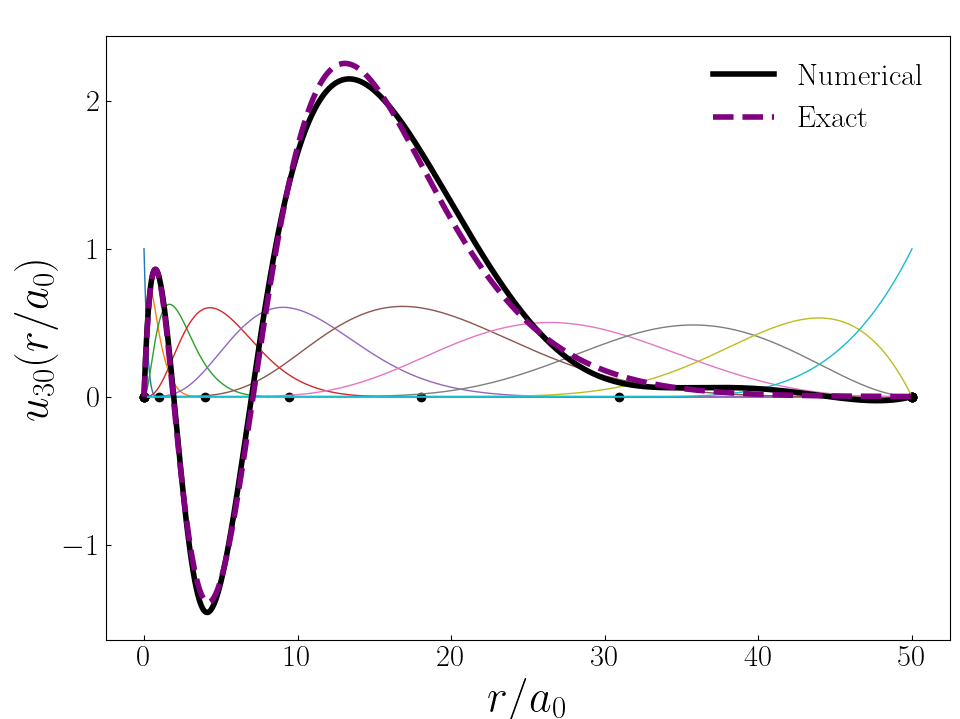
\includegraphics[scale=0.35]{u20_splines.png}
    \caption{Numerical solution to the function $P_{30}$ using B-splines. The number of splines is $M=10$ and the number of inner knot points (black points) is $N=5$.}
    \label{27apr2045}
\end{figure}
\begin{figure}[h]
    \includegraphics[scale=0.35]{errorE_2.png}
    \caption{The error of the numerical approximation of the energy $E'$ for the $(n,\ell)=(2,0)$ state for different numbers of inner knot points $N$ and order of gaussian quadrature $d$. The exact energy (in reduced units) is $-1/9$.}
    \label{27apr2138}
\end{figure}
\begin{figure}[h]
    \includegraphics[scale=0.33]{error_u20_2.png}
    \caption{The error of the numerical solution to $P_{20}$ in the point $r=13a_0$ for different number of inner knot points $N$ and order of gaussian quadrature $d$.}
    \label{27apr2139}
    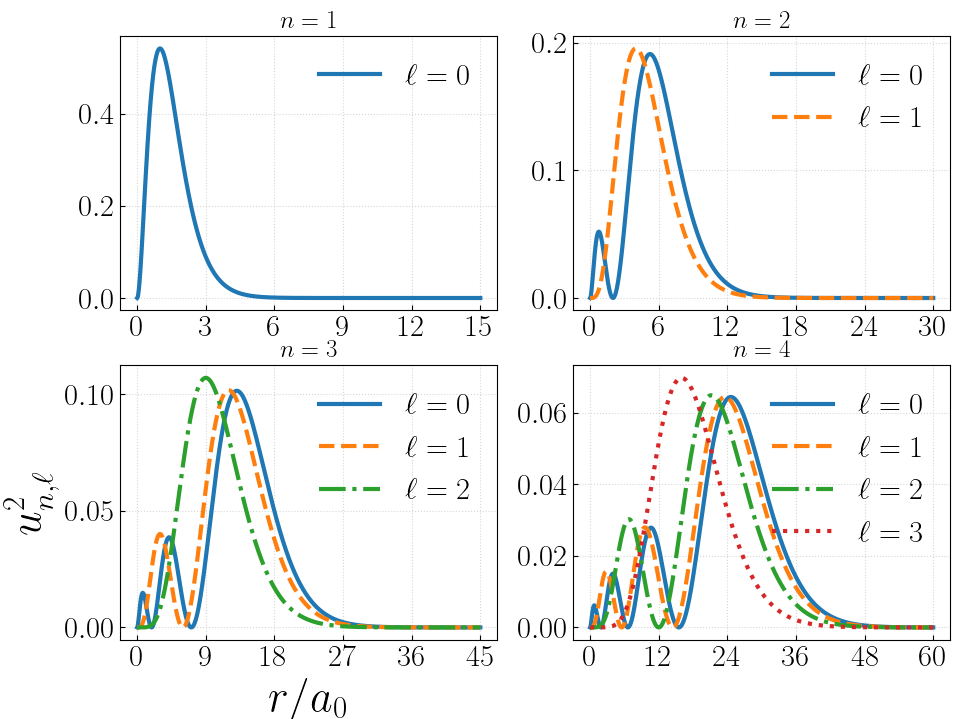
\includegraphics[scale=0.35]{Hatom.png}
    \caption{The first couple of squared reduced radial wavefunction for the Coulomb potential obtained with B-splines using 30 inner points.}
    \label{27apr2216}
\end{figure}
The method was tested on the function $P_{30}$ for the Coulomb potential with $Z = \mu/m_e = 1$. The result for just a few inner knot points ($N=5$) can be seen in figure \ref{27apr2045}. The eigenvalue from the inverse power method yielded $E'=-0.1104$ which is comparable to the exact energy $-1/9 = 0.111...$. The error at $r=13a_0$ (approximately where $P_{30}$ is  maximum) was $|u_{30}(13a_0)-P_{30}(13a_0)| = 0.10$. The order of the gaussian quadrature used to find the matrix elements was $d=4$. The error in the energy $|E'+1/9|$ and the error of the function at $r=13a_0$ were investigated for different numbers of inner knot points $N$ and order of gaussian quadrature $d$ (see figures \ref{27apr2138} and \ref{27apr2139}). As expected, the error decreases as $N$ increases but then seems to level off in the vicinity of $N = 20$. Increasing the length parameter $D$ didn't have a noticing effect on the error.

\subsection*{Results}
The first couple of $u_{n\ell}^2$ for the Coulomb potential with $Z=\mu/m_e=1$ can be seen in figure \ref{27apr2216}. These were obtained by using $N=30$ inner points and gaussian quadrature of order $d=5$. The error in the energy and in $u_{n\ell}$ at the point where $P_{n\ell}$ is maximum can be seen in table \ref{28apr0826}. 
\begin{table}[!b]
\centering
    \begin{tabular}{c c c c}
        $n$ & $\ell$ & $|E'+1/n^2|$ & $|u_{n\ell}-P_{n\ell}|_{r=r_\text{max}}$ \\ 
        \hline\hline
        1 & 0 & $8.2\cdot 10^{-9}$ &$6.0\cdot 10^{-7}$ \\ 
        2 & 0 & $8.8\cdot 10^{-8}$ &$2.6\cdot 10^{-6}$ \\ 
        2 & 1 & $2.9\cdot 10^{-8}$ &$4.2\cdot 10^{-7}$ \\ 
        3 & 0 & $2.3\cdot 10^{-7}$ &$3.7\cdot 10^{-5}$ \\ 
        3 & 1 & $1.3\cdot 10^{-7}$ &$1.6\cdot 10^{-5}$ \\  
        3 & 2 & $5.2\cdot 10^{-8}$ &$6.9\cdot 10^{-6}$ \\ 
        4 & 0 & $3.7\cdot 10^{-6}$ &$7.7\cdot 10^{-4}$ \\ 
        4 & 1 & $2.6\cdot 10^{-6}$ &$5.4\cdot 10^{-4}$ \\ 
        4 & 2 & $1.9\cdot 10^{-6}$ &$2.7\cdot 10^{-4}$ \\ 
        4 & 3 & $2.8\cdot 10^{-7}$ &$7.2\cdot 10^{-5}$ 
    \end{tabular}
    \caption{Error in energy and value of reduced radial wavefunction at the point where it is maximum from B-spline approximation. The number of innier points was $N=30$ and the order of gaussian quadrature was $d=5$.}
    \label{28apr0826}
\end{table}

The method was also used for a potential of a uniformily charged with radius $R_0=1.5a_0$ with $Z=1$ and $\mu/m_e=1$. The first couple of states for $\ell=0$ and $\ell=1$ can be seen in figure 5. A major difference compared to the Coulomb potential is that the degeneracy in $\ell$ is lifted. The ground state is also higher, $E'=-0.67$. For the $\ell=0$ states, the particle seems to be further out than in the state for the Coulomb potential. For $\ell>0$ though, the states look more the states for the Coulomb potential. This can be seen for the $\ell=1$ states and in the energy spectrum (see figure \ref{28apr1831}).
\begin{figure}[h]
    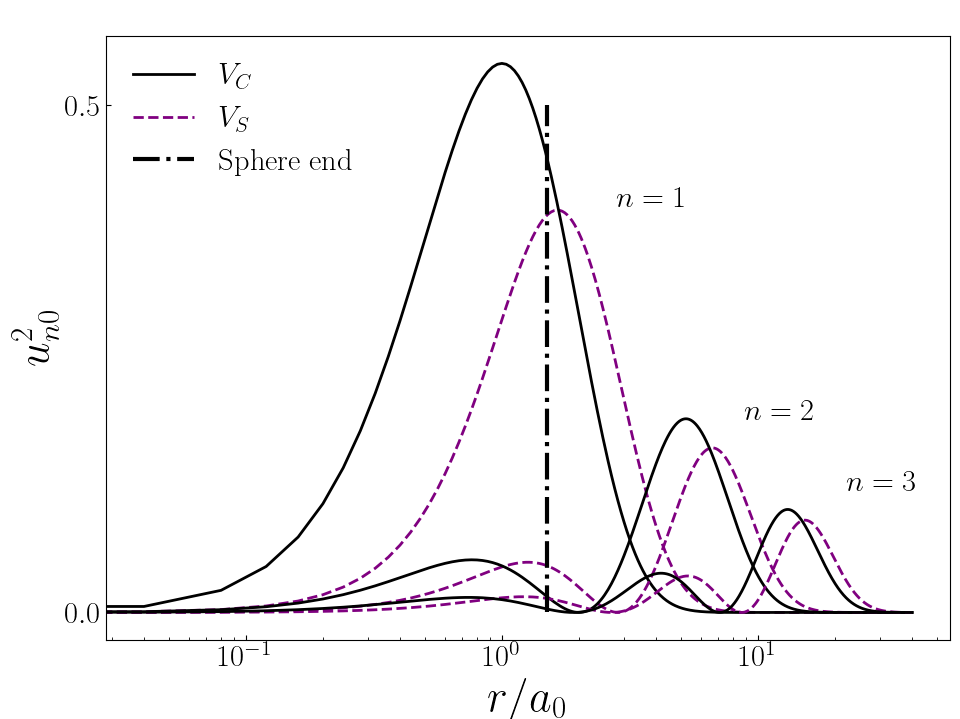
\includegraphics[scale=0.35]{sphere_l0.png}
    \label{28apr1828}
    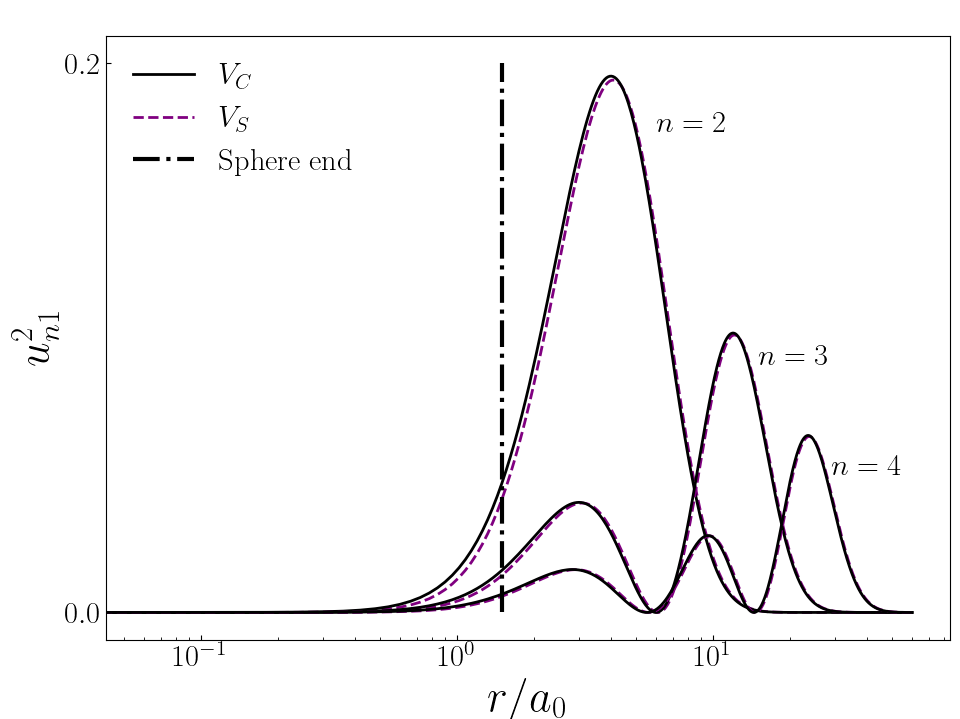
\includegraphics[scale=0.35]{sphere_l1.png}  
    \caption{The square of the reduced radial function for quantum number $\ell=0$ (top) and $\ell=0$ (bottom) with the potential from a uniformily charged sphere with radius $R_0=1.5a_0$. These were obtained using B-splines with $N=30$ inner points.}
    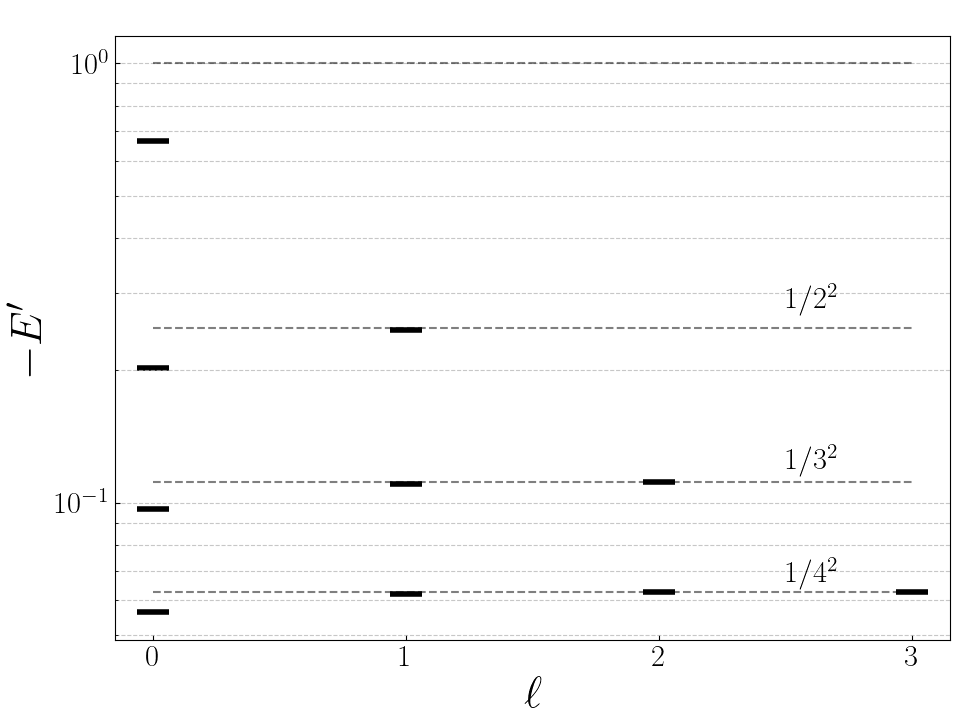
\includegraphics[scale=0.35]{spectrum.png}
    \caption{The energies $E'$ (units of 13.6 eV) and quantum numbers $\ell$ for the potential from a uniformily charged sphere of radius $R_0=1.5a_0$.}
    \label{28apr1831}
\end{figure}


\end{large}
\end{document}
